% This file was created by matlab2tikz.
%
%The latest updates can be retrieved from
%  http://www.mathworks.com/matlabcentral/fileexchange/22022-matlab2tikz-matlab2tikz
%where you can also make suggestions and rate matlab2tikz.
%
\definecolor{mycolor1}{rgb}{0.00000,0.44700,0.74100}%
\definecolor{mycolor2}{rgb}{0.85000,0.32500,0.09800}%
\definecolor{mycolor3}{rgb}{0.92900,0.69400,0.12500}%
\definecolor{mycolor4}{rgb}{0.49400,0.18400,0.55600}%
\definecolor{mycolor5}{rgb}{0.46600,0.67400,0.18800}%
%
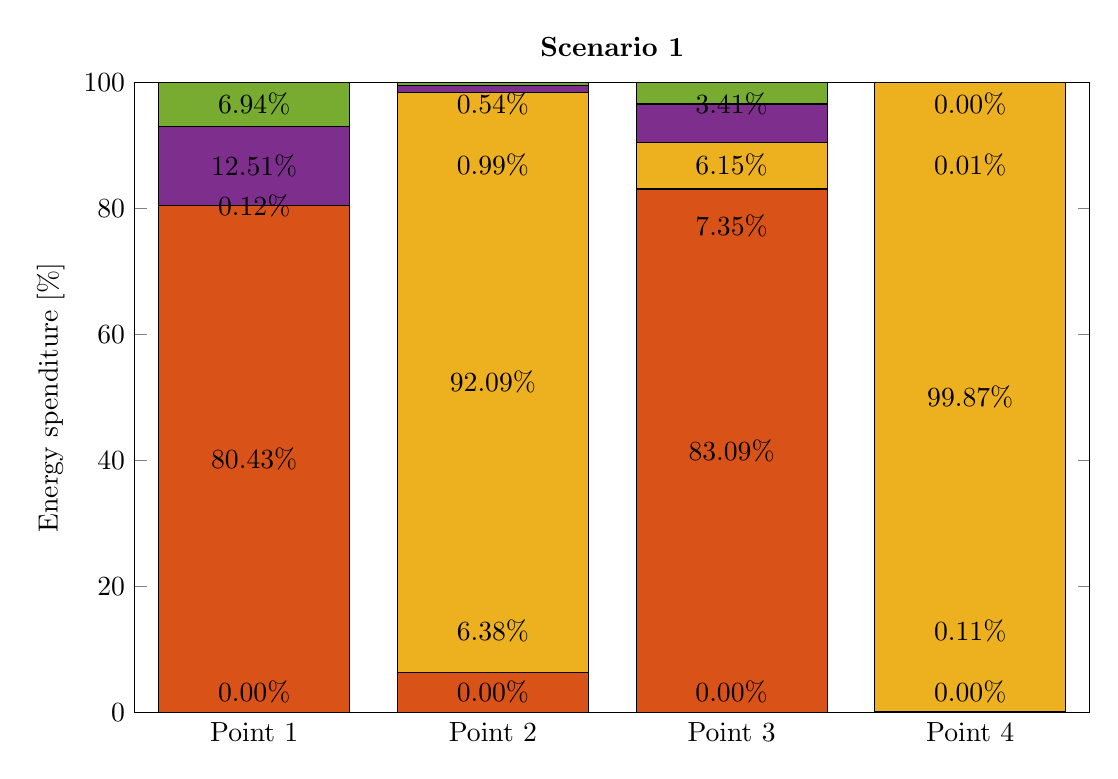
\begin{tikzpicture}

\begin{axis}[%
width=\textwidth,
height=0.66\textwidth,
at={(0.758in,0.481in)},
scale only axis,
bar width=0.8,
xmin=0.5,
xmax=4.5,
xtick={1,2,3,4},
xticklabels={Point 1, Point 2, Point 3, Point 4},
ymin=0,
ymax=100,
ylabel={Energy spenditure [\%]},
axis background/.style={fill=white},
title style={font=\bfseries},
title={Scenario 1}
]
\addplot[ybar stacked,draw=black,fill=mycolor1,area legend] plot table[row sep=crcr] {%
1	0.000416948476652553\\
2	3.30796564229127e-05\\
3	0.000204920892803428\\
4	2.78447749929594e-07\\
};
\addplot[ybar stacked,draw=black,fill=mycolor2,area legend] plot table[row sep=crcr] {%
1	80.4314444549567\\
2	6.38123100851546\\
3	83.0893922694818\\
4	0.112902369318916\\
};
\addplot[ybar stacked,draw=black,fill=mycolor3,area legend] plot table[row sep=crcr] {%
1	0.116074671790491\\
2	92.0907612628466\\
3	7.35014649609497\\
4	99.8742356375432\\
};
\addplot[ybar stacked,draw=black,fill=mycolor4,area legend] plot table[row sep=crcr] {%
1	12.51264260014\\
2	0.992721982050193\\
3	6.14968524057609\\
4	0.00835622954100753\\
};
\addplot[ybar stacked,draw=black,fill=mycolor5,area legend] plot table[row sep=crcr] ;
\node[align=center, text=black]
at (axis cs:1,40.216) {80.43\%};
\node[align=center, text=black]
at (axis cs:1,80.49) {0.12\%};
\node[align=center, text=black]
at (axis cs:1,86.804) {12.51\%};
\node[below, align=center, text=black]
at (axis cs:1,100) {6.94\%};
\node[above, align=center, text=black]
at (axis cs:2,0) {0.00\%};
\node[align=center, text=black]
at (axis cs:2,13) {6.38\%};
\node[align=center, text=black]
at (axis cs:2,52.427) {92.09\%};
\node[align=center, text=black]
at (axis cs:2,87) {0.99\%};
\node[below, align=center, text=black]
at (axis cs:2,100) {0.54\%};
\node[above, align=center, text=black]
at (axis cs:3,0) {0.00\%};
\node[align=center, text=black]
at (axis cs:3,41.545) {83.09\%};
\node[above, align=center, text=black]
at (axis cs:3,74) {7.35\%};
\node[align=center, text=black]
at (axis cs:3,87) {6.15\%};
\node[below, align=center, text=black]
at (axis cs:3,100) {3.41\%};
\node[above, align=center, text=black]
at (axis cs:4,0) {0.00\%};
\node[align=center, text=black]
at (axis cs:4,13) {0.11\%};
\node[align=center, text=black]
at (axis cs:4,50.05) {99.87\%};
\node[align=center, text=black]
at (axis cs:4,87) {0.01\%};
\node[below, align=center, text=black]
at (axis cs:4,100) {0.00\%};
\end{axis}
\end{tikzpicture}%